\chapter{CONCLUSION}

\section{Final Thoughts}
The application of generative models to any domain, has its challenges. As we saw with applying \acrshort{gan} to \acrshort{gpr}, there are some unique challenges to overcome. This thesis is a first step to further exploration of generative models for \acrshort{gpr}. From this work, it was determined that \acrshort{gan} can successfully be applied to real \acrshort{gpr} images. In addition, with the use of labeled training data, a conditional generative architecture can be applied for data augmentation. Furthermore, it was shown that a real-time classifier can be trained to detect the material of underground objects, and that this model can be improved with the incorporation of frequency domain features in classification. Moreover, With the addition of \acrshort{gan} synthesized data, we can train a classifier that detects objects with very high classification scores.

\section{Future Work}
Future research opportunities are, for the most part, infinite. However, the following are some immediate areas where improvement could be made as a continuation of this work.

\subsection{Sophisticated Object Detection in Real Time}
The first major improvement would be the addition of a more complex object detection model. Due to the desire of real time constraints, a model similar to YOLO-Lite \cite{yolo-lite} would be ideal. Figure \ref{fig:yolo-lite}, shows some preliminary work in adding YOLO to GPR data. From the figure, it is evident that more work needs to be done in this area. 

\begin{figure}[H]
    \centering
    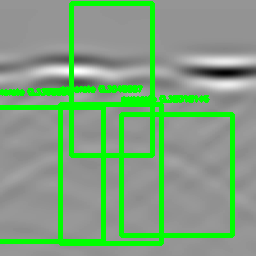
\includegraphics[width=0.6\linewidth]{figures/gpr_yolo.png}
    \caption{Preliminary Results With YOLO-Lite}
    \label{fig:yolo-lite}
\end{figure}

This would not be the first work in the field on using sophisticated object detection. However, to my knowledge, an architecture that is capable of advanced object detection in real time has not been explored in the \acrshort{gpr} space.

\subsection{Ideal GAN Architecture: gprGAN}
Recently, a major realization of the nature of \acrshort{gpr} data came to mind. Ground penetrating radar data is sequential in nature. In review of earlier material, a single B-scan consists of multiple A-scans. Therefore, it follows that an architecture could exist that encapsulates the sequential aspect of \acrshort{gpr} data. This is most important reason the proposed model architecture presented in this work, is not named gprGAN or similar, a trait commonplace in publishing work on adversarial models. A model capable of bearing the moniker gprGAN, would be able to synthesize sequences of A-scans to assemble a B-scan. Ideally, this model would be trained on one dimensional wave-forms, and have the ability to learn temporal dependencies in the segments of B-scans. Therefore, a coherent matrix of A-scans could be generated. The loss function would be a culmination of statistical distances between each A-scan in the sequence. Furthermore, it would be necessary to encompass the entire sequence of A-scans. Naturally, this sounds like a hierarchical model architecture and that could be one way of accomplishing this. In addition, it would be necessary to extending class conditioning to a multilabel problem. This would have diameter, material, and location learned independent of each other and the ability to mix these classes in conditional generation. However, a deeper exploration of this idea is necessary, but it would truly be a model capable of the title gprGAN. 